%%%%%%%%%%%%%%%%%%%%%%% file template.tex %%%%%%%%%%%%%%%%%%%%%%%%%
%
% This is a general template file for the LaTeX package SVJour3
% for Springer journals.          Springer Heidelberg 2010/09/16
%
% Copy it to a new file with a new name and use it as the basis
% for your article. Delete % signs as needed.
%
% This template includes a few options for different layouts and
% content for various journals. Please consult a previous issue of
% your journal as needed.
%
%%%%%%%%%%%%%%%%%%%%%%%%%%%%%%%%%%%%%%%%%%%%%%%%%%%%%%%%%%%%%%%%%%%
%
% First comes an example EPS file -- just ignore it and
% proceed on the \documentclass line
% your LaTeX will extract the file if required
\begin{filecontents*}{example.eps}
%!PS-Adobe-3.0 EPSF-3.0
%%BoundingBox: 19 19 221 221
%%CreationDate: Mon Sep 29 1997
%%Creator: programmed by hand (JK)
%%EndComments
gsave
newpath
  20 20 moveto
  20 220 lineto
  220 220 lineto
  220 20 lineto
closepath
2 setlinewidth
gsave
  .4 setgray fill
grestore
stroke
grestore
\end{filecontents*}
%
\RequirePackage{fix-cm}
%
%\documentclass{svjour3}                     % onecolumn (standard format)
%\documentclass[smallcondensed]{svjour3}     % onecolumn (ditto)
\documentclass[smallextended]{svjour3}       % onecolumn (second format)
%\documentclass[twocolumn]{svjour3}          % twocolumn
%
\smartqed  % flush right qed marks, e.g. at end of proof
%
\usepackage{graphicx}
%
% \usepackage{mathptmx}      % use Times fonts if available on your TeX system
%
% insert here the call for the packages your document requires
%\usepackage{latexsym}
% etc.
%
% please place your own definitions here and don't use \def but
% \newcommand{}{}
%
% Insert the name of "your journal" with
% \journalname{myjournal}
%
\newcommand{\bsat}{b_{\mathrm{sat}}}
\newcommand{\qsat}{Q_{\mathrm{sat}}}
\newcommand{\qpufa}{Q_{\mathrm{DHA}}}
\newcommand{\xsat}{x_{\mathrm{sat}}}
\newcommand{\xch}{x_{\mathrm{Chol}}}
\newcommand{\nbound}{b_{\mathrm{tot}}}
\begin{document}

\title{Nicotinic acetylcholine receptor clustering in DHA-enriched domains%\thanks{Grants or other notes
%about the article that should go on the front page should be
%placed here. General acknowledgments should be placed at the end of the article.}
}
%\subtitle{Do you have a subtitle?\\ If so, write it here}

%\titlerunning{Short form of title}        % if too long for running head

\author{K. Woods         \and
        L. Sharp \and 
        G. Brannigan %etc.
}

%\authorrunning{Short form of author list} % if too long for running head

\institute{K. Woods and L. Sharp \at
              Center for Computational and Integrative Biology, Rutgers University-Camden, Camden, NJ \\
              %Tel.: +123-45-678910\\
              %Fax: +123-45-678910\\
              %\email{fauthor@example.com}           %  \\
%             \emph{Present address:} of F. Author  %  if needed
           \and
           G. Brannigan \at
             Department of Physics, Rutgers University-Camden, Camden, NJ
}

\date{Received: date / Accepted: date}
% The correct dates will be entered by the editor


\maketitle

\begin{abstract}
The nicotinic acetylcholine receptor (nAChR) is an excitatory neurotransmitter receptor that mediates muscle functioning by forming nAChR-associated, lattice networks. At the neuromuscular junction (NMJ), synaptic and intracellular proteins, notably Agrin, MusK, and rapsyn, ultimately stabilize these highly dense networks. Experimental evidence suggests that cholesterol-rich domains, known as lipid rafts, facilitate signaling among Agrin-Musk and rapsyn, and their presence is essential for healthy nAChR clustering. In spite of their importance, the structural and functional mechanisms of lipid domains are currently unknown. Alongside cholesterol, Docosahexaenoic acid (DHA) omega-3 fatty acids are prevalent at the NMJ, correlate with domain formation, and strongly promote neuronal health. In the present study, we computationally explored the role of DHA on nAChR clustering in the presence and absence of lipid domains. Within coarse-grained (CG) model membranes, nAChRs consistently partitioned into flexible, liquid-disordered domains; boundary lipids were rich in DHA regardless of the number of nAChR molecules, but preventing domain formation also reduced the likelihood of these acyl chains aggregating around nAChR. Taken together, our findings suggest that by inducing domain formation in membranes, DHA plays a critical role in the early stages of nAChR oligomerization.
\keywords{Nicotinic acetylcholine receptor (nAChR) \and Polyunsaturated fatty acids (PUFAs) \and Domain formation \and Neuromuscular Junction (NMJ) \and Lipid-protein interactions \and Lipid rafts \and Docosahexaenoic acid (DHA)}
% \PACS{PACS code1 \and PACS code2 \and more}
% \subclass{MSC code1 \and MSC code2 \and more}
\end{abstract}

\section{Introduction}
\label{intro}
%Your text comes here. Separate text sections with
\subsection{Neuromuscular nicotinic acetylcholine receptors (nAChRs) and their lipid interactions}
\label{sec:1}
The muscle-derived nicotinic acetylcholine receptor (nAChR) (PDB id-2BG9)\cite{Unwin2005} is the most abundant neurotransmitter receptor at the neuromuscular junction (NMJ) in most vertebrates, including humans \cite{Albuquerque2009}. Within the postsynaptic membrane, nAChRs cluster in high densities (10,000 per $\mu$m$^{2}$) to properly activate the skeletal muscle\cite{Ramarao1998,Breckenridge1972}. As a major transmembrane protein, nAChR depends upon a highly specific lipid environment to maintain functionality. Experimentally, lipids influenced nAChR activity by stabilizing its open and closed states\cite{Criado1982}, channel gating properties\cite{daCosta_A_2013}, and position within the membrane\cite{Almarza2014}. It is important to understand how changes in lipid environment impact nAChR's structure and activity, given that lipids can change in response to aging and disease \cite{Yadav2014}. 

Over the past few decades, considerable progress has been made in uncovering lipid sensitivities associated with nAChR \cite{Criado1982}. In a majority of experiments, researchers have prioritized cholesterol over other membrane lipids \cite{Narayanaswami1993,Leibel1987,Marsh1978,POPOT1978}. Early studies revealed that, when reconstituted into membrane mixtures, nAChR failed to conduct cations across the lipid bilayer unless cholesterol was present \cite{Fong_Correlation_1986,Sunshine_Lipid_1992,Butler1993,Fong_Stabilization_1987,Corrie_Lipid_2002}. 
%\subsection{Subsection title}
%\label{sec:2}
%as required. Don't forget to give each section
%and subsection a unique label (see Sect.~\ref{sec:1}).
\subsection{nAChR clustering in association to lipid rafts}
More recently, researchers have examined the effects of membrane dynamics on nAChR organization\cite{Baenziger2015,Bruses2001,Marchand2002a,Oshikawa2003,Pato2008,Zhu2006a,Baenziger2017,Baenziger2017,Barrantes2007,Barrantes2000,Barrantes2010,Bermudez2010,Perillo2016,Wenz2005,Borroni2016,Unwin2017}. In-vitro studies\cite{Barrantes2007, Barrantes2010} indicate that nAChRs form larger aggregates upon cholesterol depletion. Experimental evidence suggest that cholesterol-rich lipid domains, known as lipid rafts, facilitate clustering of nAChRs\cite{Campagna2006,Marchand2002a,Pato2008}. 
More specifically, after disrupting lipid raft formation, Zhu observed a significant loss nAChR clusters in-vitro\cite{Zhu2006a}. In the mature neuromuscular membrane, nAChRs are linked by the intracellular anchoring protein, rapsyn, which bridges receptors together at their bases \cite{Zuber2013a}. According to fluorescent studies\cite{Marchand2002a}, lipid rafts mediate the association between rapsyn and neighboring nAChR molecules. In the mid-2000's, Willmann (2006) and Stetzkowski-Marden (2006) proposed that lipid rafts can stabilize receptor networks and may even provide a localized environment for nAChR \cite{Willmann2006,Stetzkowski-Marden2006}. 




Domain formation can occur when the following conditions are satisfied: the membrane must contain a sufficient concentration of cholesterol, unsaturated fatty acids, and a molecule that interacts closely with cholesterol such as saturated fatty acids or sphingomyelin\cite{Feller_Acyl_2008,Yeagle2016115}. In neuromuscular membranes, intrinsic domain formation is dependent upon several lipid species, including the widely influential omega-3 fatty acids. One omega-3 in particular, Docosahexaenoic acid (DHA), is prevalent in the native neuromuscular membrane and is strongly associated with flexible and well-defined domains \cite{Turk2013,shaikh_dumaual_castillo_locascio_siddiqui_stillwell_wassall_2004}. Additionally, DHA is a major contributor to brain functioning, motor activity, and cardiac health; however, its specific effects on neuromuscular health are poorly understood \cite{12439486320170901,S000930840800032720080101,Georgieva2015}. 


Recently, Sharp et. al (2018)\cite{Sharp2018} computationally investigated nAChR-lipid interactions in mixtures containing polyunsaturated fatty acids (PUFAs). Contrary to expectations, nAChR consistently preferred a local lipid environment characterized by PUFAs rather than cholesterol, especially long-chained omega-3s, such as DHA. While cholesterol occupied the transmembrane gaps of nAChR, PUFAs were even more likely to embed, regardless of their phospholipid headgroup. 


The present study adopts a similar approach to Sharp et. al (2018), with a particular focus on nAChR-associated clustering. Through molecular dynamics simulations, we investigate nAChR lipid preferences and clustering behavior in membranes with and without domains. For this study, we tested three major hypotheses: 1) Membrane organization affects nAChR boundary lipid specificity: when PUFA chains are prevented from forming PUFA rich domains, their prevalence among nAChR boundary lipids will be significantly reduced. 2) Domain formation will indirectly facilitate the clustering of nAChRs, by inducing partitioning preferences and restricting diffusion within the membrane. 3) Within a dimer, we will observe sequence preferences in facing subunits.
%\paragraph{Paragraph headings} Use paragraph headings as needed.
\section{Methods}
\subsection{System setup}

We constructed 18 coarse-grained (CG) molecular dynamics simulations containing 2-4 nAChRs (3 replicas per system), derived from the Torpedo electric organ\cite{Unwin2005}. One membrane had intrinsic domain formation, due to its fully saturated and fully unsaturated phospholipids: 35:35:30 Di-palmitoyl phosphatidylcholine (DPPC): Di-docosahexaenoyl\\ phosphatidylcholine (DHA-PC): Cholesterol. In a second composition, domain formation was prevented by using a mixture of hybrid lipids, each with one DHA and one saturated tail: 70:30 1-palmitoyl-2-docosahexaenoyl-phosphatidylcholine (PUPC): Cholesterol. \cite{Marrink2007}




The Martini CG force field allowed us to observe large-scale membrane interactions that are inaccessible through atomistic approaches (AA); such interactions include domain formation, protein partitioning, and protein clustering. By using a CG model, we could run simulations for longer length and time scales, with systems approaching equilibrium at approximately 2 $\mu$s.  \cite{Marrink2007}
We converted protein structures into coarse-grained models using the Martini script "martinize.py", mapping four non-hydrogen atoms to one CG interaction. We constructed and assembled our protein-bilayer systems using  the Martini script, "insane.py", specifying a box size of 44x44x22nm$^{3}$ for multiple-protein systems, respectively.  \cite{Marrink2007}
 






\subsection{Simulation details}
Simulations were run using the Martini 2.2 force field parameters and the Gromacs 5.1.2 simulation package.\cite{Marrink2007, Pronk2013} Each simulation consisted of two phases: energy minimization and molecular dynamics. For each system, we ran two consecutive equilibrium simulations for 10,000 steps at a 0.001 ps time-step.  


Harmonic restraints between backbone atoms were imposed to preserve nAChR conformation. More specifically, we applied an elastic force constant of 750 kJ/mol and set lower and upper bounds on the bond with lengths 0.9 nm and 1.6 nm, respectively\cite{Marrink2007, Pronk2013}.  

 
The molecular dynamics simulations ranged between 3 and 10 $\mu$s at a 0.025 ps time-step. Simulation temperature and pressure were kept constant at values of 323 K and a reference pressure of 1 bar. The isotropic pressure coupling compressibility constant was maintained at 3.0 $\times {10^{-5}}$ bar$^{-1}$ .



% rephrase using the information from Liam's paper below (commented out)

%All simulations were run using a isothermal-isobaric (NPT) ensemble, with a Berendsen thermostat of 323 K and a temperature coupling constant of 1 ps, as well as isotropic pressure coupling with compressibility set to $3\times 10^{-5}$ bar$^{-1}$ and a pressure coupling constant set to 3.0 ps.

\subsection{Analysis}
We visualized and imaged all simulation results using the Visual Molecular Dynamics (VMD) program \cite{HUMP96}. First, we quantified the degree of protein partitioning within a lipid domain by counting the number of $b$ boundary lipids and comparing it with its expectation in a randomly mixed membrane. In the case of saturated lipids, the metric $Q$ can be written as follows:


\begin{equation}
    \begin{aligned}
      \qsat\equiv \frac{1}{\xsat}\left\langle\frac{  \bsat }{\nbound }\right\rangle-1,\\
    \end{aligned}
    \label{eq:Q}
  \end{equation}


where $b_{sat}$ is the number of saturated boundary lipids, $b_{total}$ represents the total number of boundary lipids, and $x_{sat}$ represents the expected value for saturated boundary lipids, based on the initial, randomly-mixed composition.   
%Similarly, we constructed two-dimensional distributions of boundary lipids over a series of polar bins. This order parameter is defined as follows:



 % \begin{equation}
  %    \rho_{B,i}=\left\langle \frac{n_{B,i}}{A_{i}}\right\rangle \\        
   % \label{eq:Embedded}
  %\end{equation}
  %where $n_{B,i}$ is the number of lipid $b$ found within bin$_i$ and $A_i$ represents bin area.
  

Next, we directly compared the tendency for nAChR to self-dimerize in the presence or absence of lipid domains. For each simulation, we calculated the center of mass (COM) separating unique pairs of proteins, and computed the average pairwise distance per time-step. We calculated the average pairwise distance between all proteins in the system as:    


\begin{equation}\label{eq:dimer}
\left\langle D \right\rangle = \frac{\sum D_{ij}}{N_{p}}
\end{equation}

where $D_{ij}$ is the distance between the $i$th protein and the $j$th protein, and $N_{p}$ refers to the number of unique protein pairs. 



Lastly, we calculated the percentage of time that a subunit pair faced one another with the following equation: 

\begin{equation}\label{eq:subunit}
F_{x,y} = 100\cdot \frac{n_{x,y}}{n_d}
\end{equation}

. Here, $n_{x,y}$ represents the number of frames in which subunits "x and y" are the closest and $n_d$ is the total number of frames that the two proteins cluster together (satisfying a cutoff of 200 {\AA}).

\section{Results}

\subsection{nAChR boundary lipid preferences}\label{sec:lipids}

For simulations containing 2-4 nAChRs, we measured the fraction of boundary lipids that occupy the outer perimeter of the protein. Using Equation \ref{eq:Annular}, we constructed distributions of annular acyl chains across all systems, with data collected from 2000 to 3000~ns trajectories, respectively. As shown in Figure \ref{fig:Figure2}, in domain-forming compositions DHA occupied the largest proportion of annular lipids (85 \%) followed by saturated lipids (15 \%) and cholesterol (5 \%). For polyunsaturated lipids and cholesterol, the observed annular concentrations were significantly different than the values expected based on their starting compositions, with annular DHA higher than the bulk concentration and annular cholesterol less than the bulk concentration.  In hybrid mixtures, nAChRs no longer exhibited acyl chain preferences, and acyl chain distributions better fit the expected annular ratios in a randomly mixed membrane (See Figure \ref{fig:Figure2}).

\begin{figure}[h]
\center
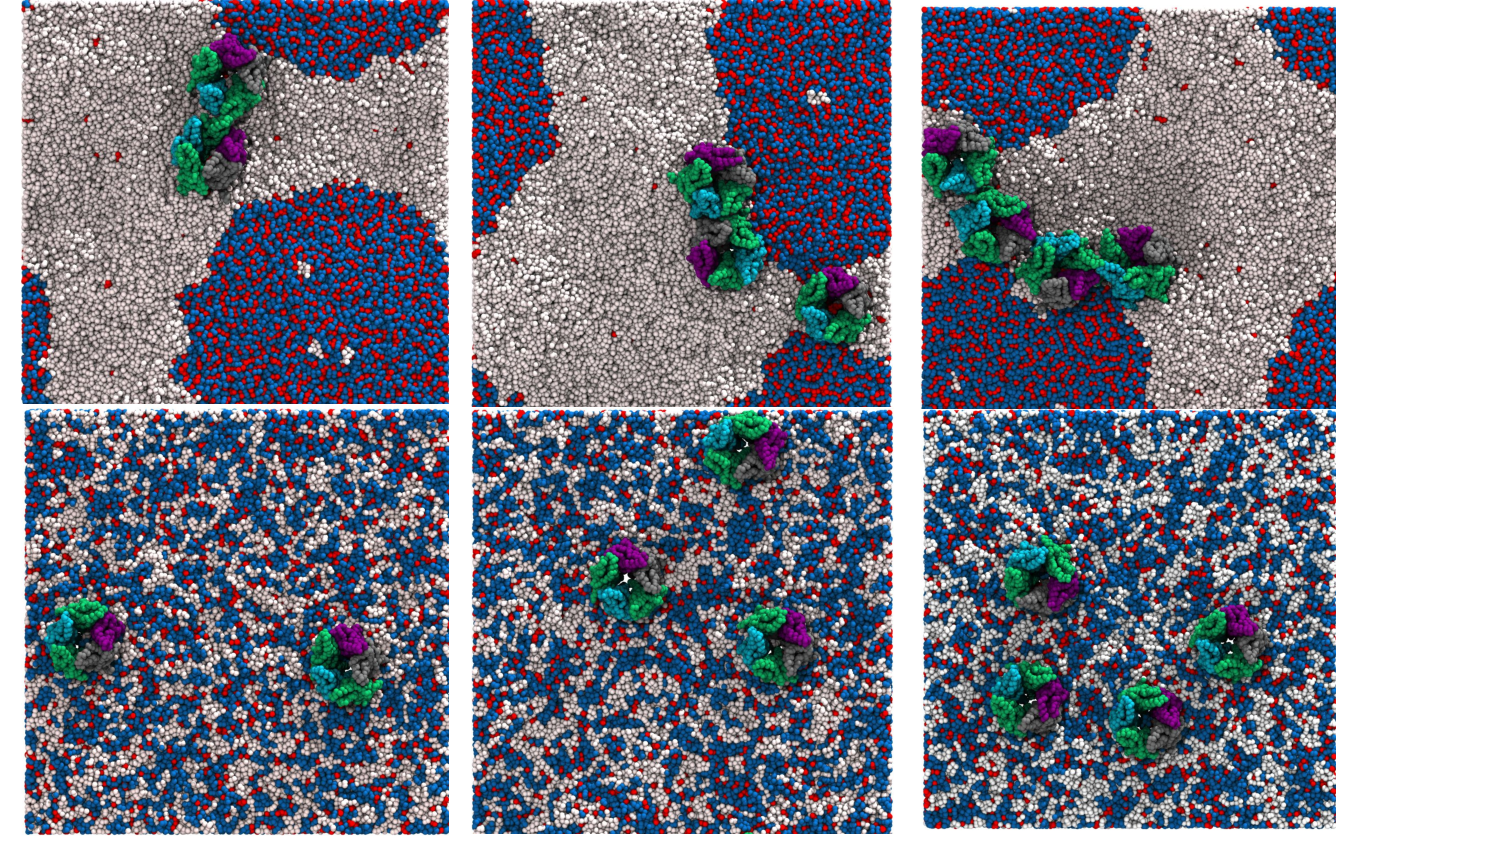
\includegraphics[width=\linewidth,trim={0cm 0cm 0cm 0cm}]{Figure3}
\caption[Protein clustering in domain-forming (top row) and hybrid (bottom row) membranes.]{{\bf Protein clustering in domain-forming (top row) and hybrid (bottom row) membranes.} nAChRs were colored by subunit ($\alpha:green,\beta:purple,\delta:gray,\gamma:cyan$), and lipids by acyl chain (DHA: white, saturated: blue, and cholesterol: red). Clustering of nAChRs on the borders of lipid rafts is visible in the domain-forming membranes.}
\label{fig:Figure4}
\end{figure}



\begin{figure}[h]
\centering
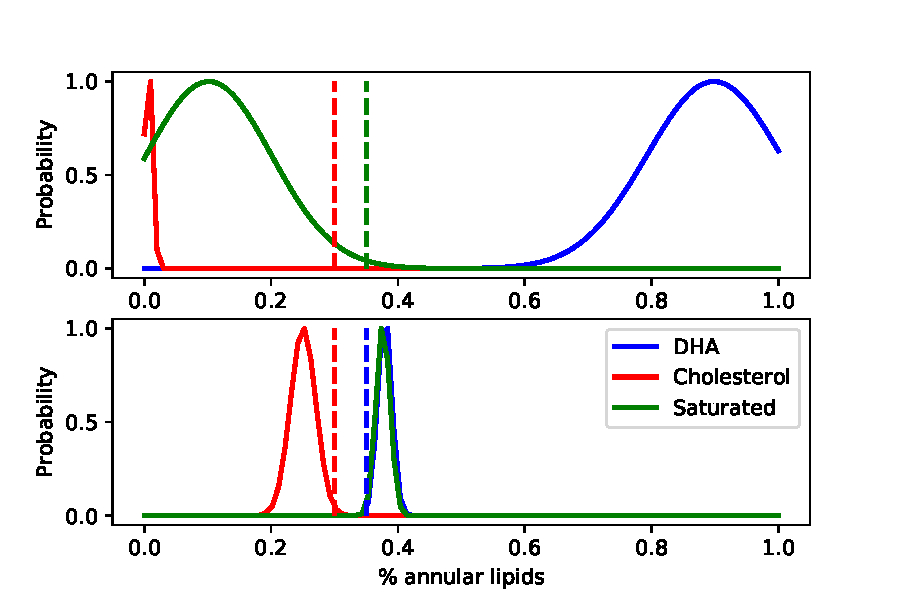
\includegraphics[width=.99\linewidth,trim={0cm 0cm 0cm 0.5cm}]{Figure2_prob}
\caption[nAChR boundary lipid preferences.]{{\bf nAChR boundary lipid preferences.} Probability distribution function showing the distribution of lipid concentrations in close proximity to nAChR (10-35 {\AA}  from the the center M2 helices). Top depicts membranes with domain formation. Bottom depicts membranes without domain formation. Distributions reflect aggregate data for systems containing two, three, and four nAChRs. Dashed lines represent expected boundary ratios for a randomly-mixed membrane, based on overall lipid composition.}
  \label{fig:Figure2}
\end{figure}



%Next, using Equation \ref{eq:Embedded}, we calculated the average density of each lipid species within 5~nm from the center of nAChR; these data represented the average non-annular lipid concentrations buried within the transmembrane bundle. In Figure \ref{fig:Figure3}, we plotted densities based on headgroup, given that both compositions have idenitical headgroup concentrations (30:PC, 30:PE, 30:CHOL, 10:PS). All data were normalized to account for differences in headgroup concentrations, as well as membrane thicknesses.


%In both domain-forming and hybrid membrane compositions, PS (blue) and PE (magenta) phospholipids were predominately concentrated near the innermost and outermost transmembrane helices, located respectively  approximately 1 nm and 4 nm from the center of mass of nAChR. However, in domain-forming membranes these lipids exhibited a greater affinity for M2 and M4. Meanwhile, cholesterol occupies only 15 \% of non-annular sites in the presence of domains, and up to 12.5 \% in the absence of domains, as seen in Figure \ref{fig:Figure3}; these values show cholesterol relatively depleted throughout the transmembrane bundle compared to its annular concentration shown in Figure~\ref{fig:Figure2}. Across all systems, PC phospholipids were least likely to embed, with a maximum concentration of 12 \% over the 5 nm range. Please see Figure ~\ref{fig:Figure3} for more information.



%\begin{figure}[H]
%\center
%  \subfigure[Domains]{
%    \includegraphics[width=.8\linewidth]{Figure3a}
%    \label{domains}}
%  \subfigure[No domains]{
%    \includegraphics[width=.8\linewidth]{Figure3b}
%    \label{no domains}}
%\caption[Nonannular lipid-binding.]{{\bf Nonannular binding of lipids based on headgroup.} Lipid densities within 5 nm of the nAChR COM (Top: Domain-forming, Bottom:Hybrid). Lipids were colored by headgroup in both compositions (PC: green, PE: purple: CHOL: red, PS: blue).  All data were normalized to account for differences in headgroup concentrations, as well as membrane thicknesses. }
%\label{fig:Figure3}
%\end{figure}







\subsection{nAChR clustering in the presence and absence of lipid domains} \label{sec:clustering}
To better characterize the clustering nAChRs, we constructed two distributions of pairwise distances for each membrane composition, using equation \ref{eq:dimer} above. In figure \ref{fig:Figure6}, distributions reflect aggregate data averaged over simulations from 2000 to 3000 ns. In domain-forming membranes, the majority of nAChR pairs were close together, with a mean distance around 125 {\AA}. In contrast, for hybrid membranes, nAChRs were farther apart, averaging around 225 {\AA}.  


\begin{figure}[h]
\centering
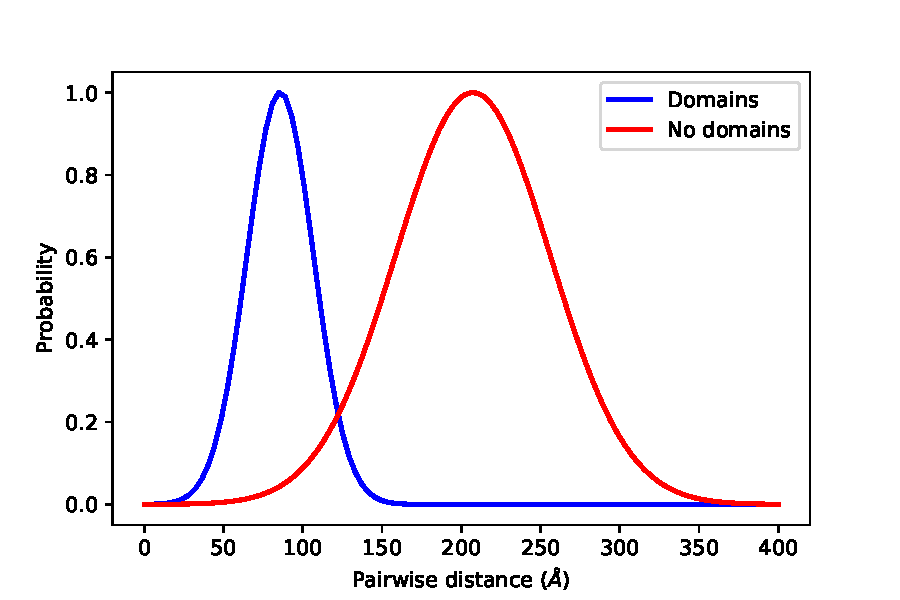
\includegraphics[width=\linewidth,trim={0cm 0cm 0cm 0cm}]{Figure3_prob}
\caption[Pairwise distance distribution across multi-protein systems.] {{\bf Pairwise distance distribution across multi-protein systems.} Distribution of average pairwise distances across all simulations. Data collection began at 2000 ns into each trajectory and ended at 3000 ns, respectively. }
\label{fig:Figure6}
\end{figure}


%In Figure ~\ref{fig:Figure5}, three subplots depict the average distance between pairs of distinct proteins, in systems containing two, three, or four nAChRs. Across 1500-4000 ns trajectories, the average distance between distinct pairs of proteins is smaller in membranes with well-defined domains, compared to those lacking domains. 


In the majority of domain-forming membranes, we observed the formation of nAChR dimers along domain interfaces. Along domains, a majority of pairwise distances  fell within 100-150 {\AA} by 3000 ns (see Figure \ref{fig:Figure4}). This trend persisted within and across individual simulations, regardless of protein concentration or the size and shape of domains.





%\begin{figure}[H]
%	\center
%	\includegraphics[width=\linewidth]{Figure5}
%\caption[Average pairwise distance between nAChR molecules over time.] {{\bf Average pairwise distance between nAChR molecules over time.} Pairwise distance vs time for 12 multi-protein systems.  Here pairwise distance is the average distance between the centers of mass across pairs of proteins.}
%\label{fig:Figure5}
%\end{figure}


















\subsection{Closest subunits across dimerizing proteins}
Our final analysis calculated the distance between nAChR subunit pairs for dimerizing proteins, using equation \ref{eq:subunit}, focusing on identifying the closest pair among the 15 possible subunit combinations. Among all simulations, the nAChR $\alpha_{\delta}$ subunit most frequently formed the closest pair, pairing with $\delta$, and $\gamma$ subunits well above expectation (10-15 \%) in both domain-forming and hybrid membranes. In domain-forming membranes, the most frequent closest subunit pairs were $(\alpha_\delta, \delta)$ and $(\alpha_\delta, \gamma)$, each appearing in more than 15 \% of simulations. In hybrid membranes, in addition to the $\alpha_{\delta}$ subunits mentioned above, $(\alpha_\gamma, \gamma)$ were among the closest subunits at a level above expectation. On the other hand, the nAChR $\beta$ subunits formed the fewest subunit pairs, falling well below the expectation value for each pair. Please refer to Figure ~\ref{fig:Figure7} for a heat-map of these data.   


\begin{figure}[h]
	\center
	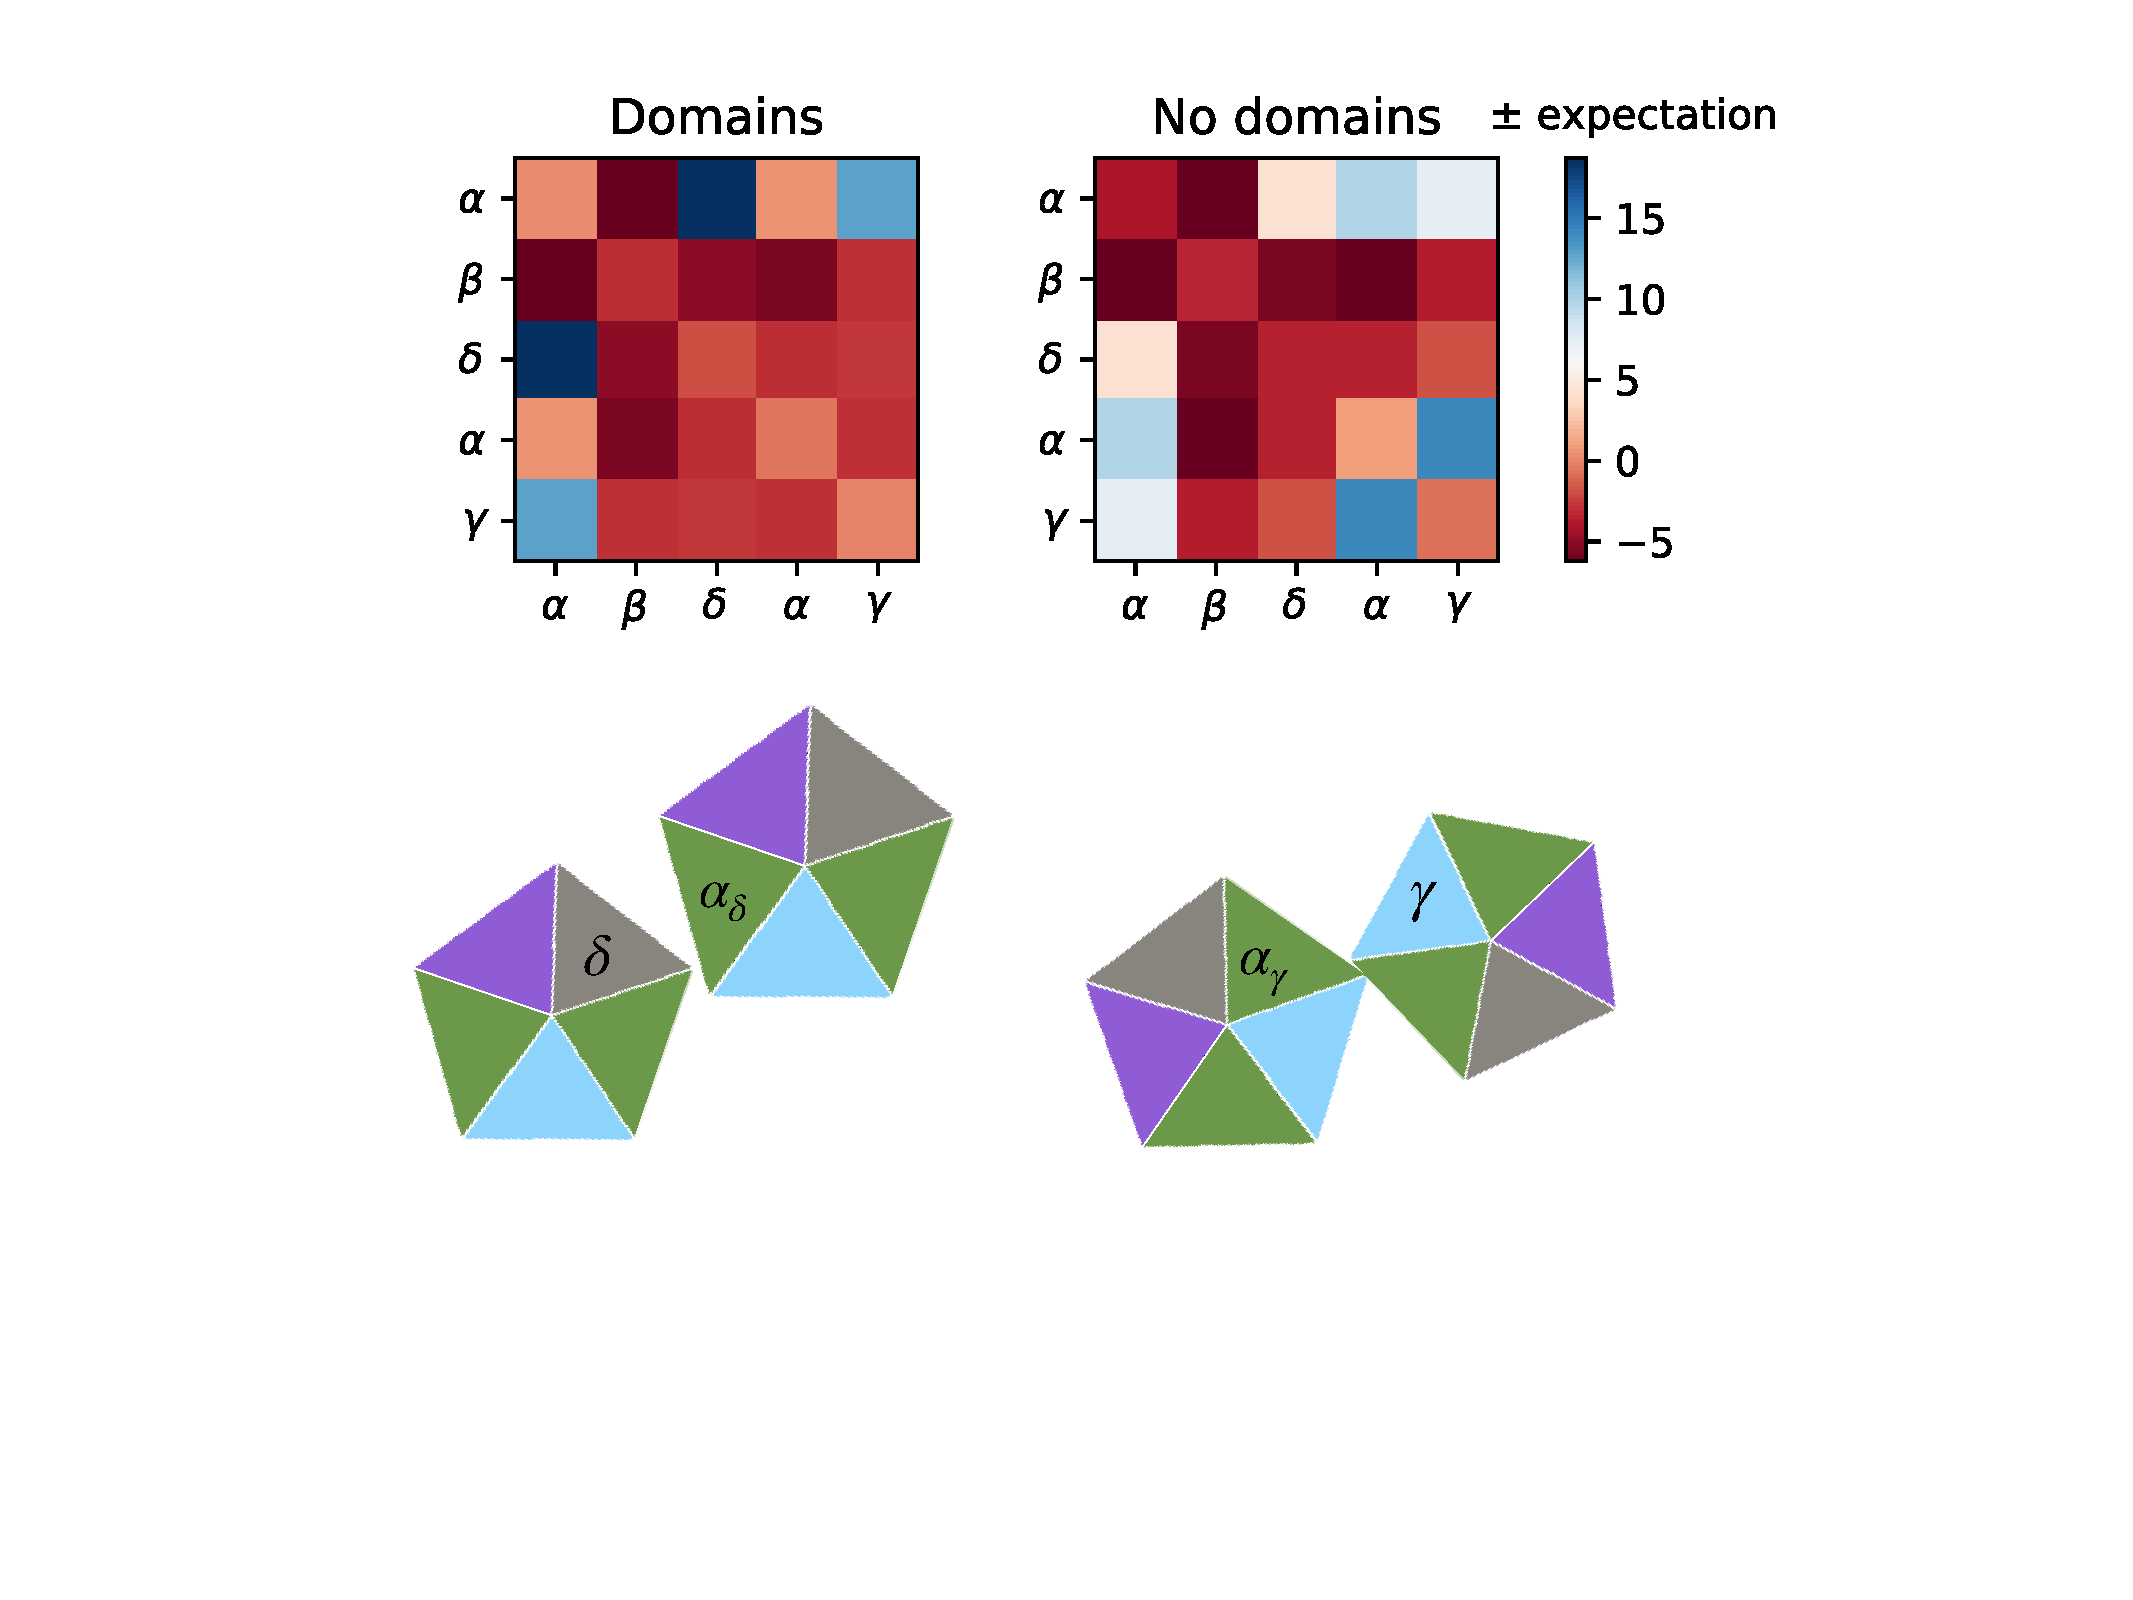
\includegraphics[width=1.0\linewidth, trim={3cm 8cm 3cm 8cm}]{Figure4}
\caption[Subunit pairs among dimerizing proteins]{{\bf Subunit pairs among dimerizing proteins.} Heat-map showing the likelihood that two subunits were closest together among dimerizing proteins (200 {\AA} threshold). Distinct subunits are expected to form the closest pair 8 \% of the time, while identical subunits are expected to dimerize only 4 \% of the time. Each color on the heatmap represents a specific deviation from the pair's expectation value, ranging from -5 (red) to 15 (blue).  }
\label{fig:Figure7}
\end{figure}



\section{Discussion}


Found primarily in fish oil, DHA has been generally associated with enhanced cognitive functioning, as well as benefits in cardiac health and disease prevention \cite{12439486320170901}. 
As stated previously, DHA is an omega-3 fatty acid  found primarily in the brain, synapses, and the Torpedo electric organs, all of which are native membranes for human nAChR. While DHA is implicated in human health and disease, its interactions with critical membrane proteins, such as nAChR, have been largely overlooked in previous studies. Consistent with MD-CG simulations using one nAChR \cite{Sharp2018}, multiple nAChRs continue to prefer the liquid-disordered phase containing long-chain omega-3 fatty acids. More specifically, nAChRs partitioned into DHA-enriched domains. 

%%

%While it is well-established that cholesterol leads to a gain-of-function in nAChR, adding anionic lipids like POPA to a purely POPC or POPC:CHOL reconstitution mixture also results in significant gain-of-function, causing some researchers to suggest anionic lipids are required for functional conformations of nAChR \cite{Corrie_Lipid_2002}. If so, we might expect anionic lipids (such as the DHA-PS used here) to have a higher probability of being in the nAChR boundary than zwitterionic lipids. Instead, we find that anionic lipids and zwitterionic lipids (PE headgroups) had similar affinities for nAChR's TMD. It is important to emphasize that in domain-forming membranes, PS and PE phospholipids both had DHA acyl chains and their probabilities of embedding were much higher compared to those in hybrid mixtures (See Figure \ref{fig:Figure3}). While cholesterol embedded throughout the nAChR transmembrane bundle, DHA-PS and DHA-PE occupied these non-annular sites in higher concentrations. This supports the hypothesis that, alongside cholesterol, PUFAs can provide additional support to nAChR structural and functional integrity, as hypothesized by Sharp et. al (2018) \cite{Sharp2018}.


To our knowledge, previous studies have not included PUFAs in their membrane mixtures, which may affect the interactions between lipids and the nAChR ion pore. \cite{Fong_Correlation_1986,Sunshine_Lipid_1992,Butler1993,Fong_Stabilization_1987,Corrie_Lipid_2002}. Our data show that by inducing domain formation in membranes, DHA leads to the clustering of nAChRs in the flexible, liquid-disordered phase and supports their boundary acyl chain preference for PUFAs (Figure \ref{fig:Figure2}). Without domain formation, since hybrid lipids only have one DHA chain each, DHA cannot aggregate around nAChRs to the same degree. 


%Additionally, by clustering along specific nAChR subunits, neuromuscular nAChRs  may also depend on protein sequence for the early stages of nAChR dimerization. 
Pentameric ligand-gated ion channels, such as nAChR and GABA-A, have retained function for millions of years and are found in many species - from bacteria to humans; however, heteromers, which include $\gamma$ or $\delta$ subunits, are found in higher-level organisms and between synapses \cite{Jaiteh2016}. In our simulations, $\delta$ and $\gamma$ subunits promoted oligomerization of muscle-type nAChRs. This preference in subunit pairs may indicate an essential role for heteromerization in pLGIC oligomerization within the nervous system. Building on this work, we aim to expand the scope of our computational models, with special consideration to the individual effects of membrane elasticity, protein concentration, and pLGIC sequence on nAChR oligomerization.  







% For one-column wide figures use
%\begin{figure}
% Use the relevant command to insert your figure file.
% For example, with the graphicx package use
%  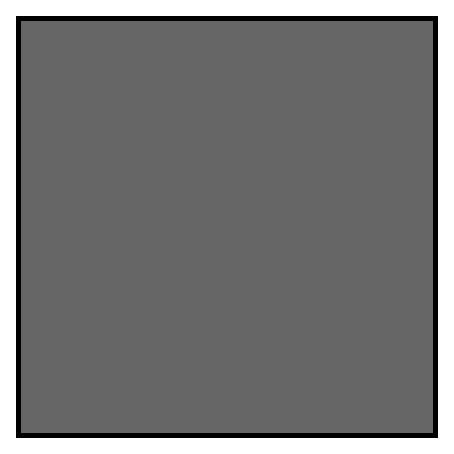
\includegraphics{example.eps}
% figure caption is below the figure \caption{Please write your figure caption here}
%\label{fig:1}       % Give a unique label
%\end{figure}
%
% For two-column wide figures use
%\begin{figure*}
% Use the relevant command to insert your figure file.
% For example, with the graphicx package use
 % 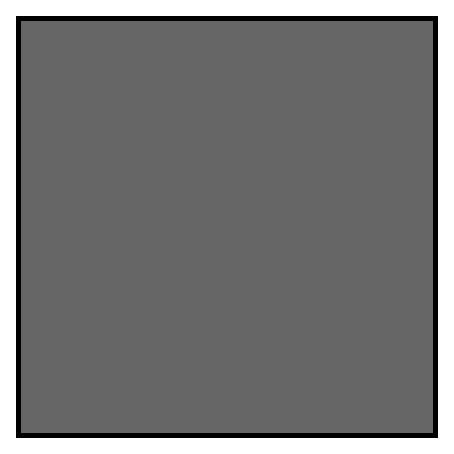
\includegraphics[width=0.75\textwidth]{example.eps}
% figure caption is below the figure
%\caption{Please write your figure caption here}
%\label{fig:2}       % Give a unique label
%\end{figure*}
%
% For tables use
%\begin{table}
% table caption is above the table
%\caption{Please write your table caption here}
%\label{tab:1}       % Give a unique label
% For LaTeX tables use
%\begin{tabular}{lll}
%\hline\noalign{\smallskip}
%first & second & third  \\
%\noalign{\smallskip}\hline\noalign{\smallskip}
%number & number & number \\
%number & number & number \\
%\noalign{\smallskip}\hline
%\end{tabular}
%\end{table}
%

%\begin{acknowledgements}
%If you'd like to thank anyone, place your comments here
%and remove the percent signs.
%\end{acknowledgements}

% BibTeX users please use one of
%\bibliographystyle{spbasic}      % basic style, author-year citations
%\bibliographystyle{spmpsci}      % mathematics and physical sciences
%\bibliographystyle{spphys}       % APS-like style for physics
%\bibliography{}   % name your BibTeX data base  

% Non-BibTeX users please use
%\begin{thebibliography}{}
%
% and use \bibitem to create references. Consult the Instructions
% for authors for reference list style.
%
%\bibitem{RefJ}
% Format for Journal Reference
\bibliographystyle{spmpsci}
\bibliography{BIBx.bib}
%\end{thebibliography}

\end{document}
% end of file template.tex

